\section{Introduction}

Nowadays, malware usually uses HTTP protocol to connect suspicious host for data leakage and exfiltration, because it's a common network channel that Intrusion Detection/Prevention Systems (IDS/IPS) never block the HTTP traffics. Therefore, malware tries to hide their penetrations in the HTTP traffic to evade the detections in Figure ~\ref{fig:attack}. In the previous research, there are many botnet using HTTP protocl to communicate with the C\&C server for waiting command instead of IRC channel \cite{gu2008botsniffer}. However, the proposed method in the past that uses fingerprint to detect malware hide in outbound HTTP traffics \cite{bortolameotti2017decanter}, and which can't efficiently detect malware when hacker generates counterfeit fingerprints.  

The main idea concept of fingerprint is around the HTTP headers. But, as we know, hacker can use exploit tool or library to eaily modify the contents of a HTTP header. Previous research also indicates that malware uses modified HTTP header to evade the latest detections system \cite{grill2014malware}, and which points out most malware using browser-like user-agent since browser's connection behavior is various and complex. Therefore, we represent the problem define as following:

\begin{figure}[!t]
\centering
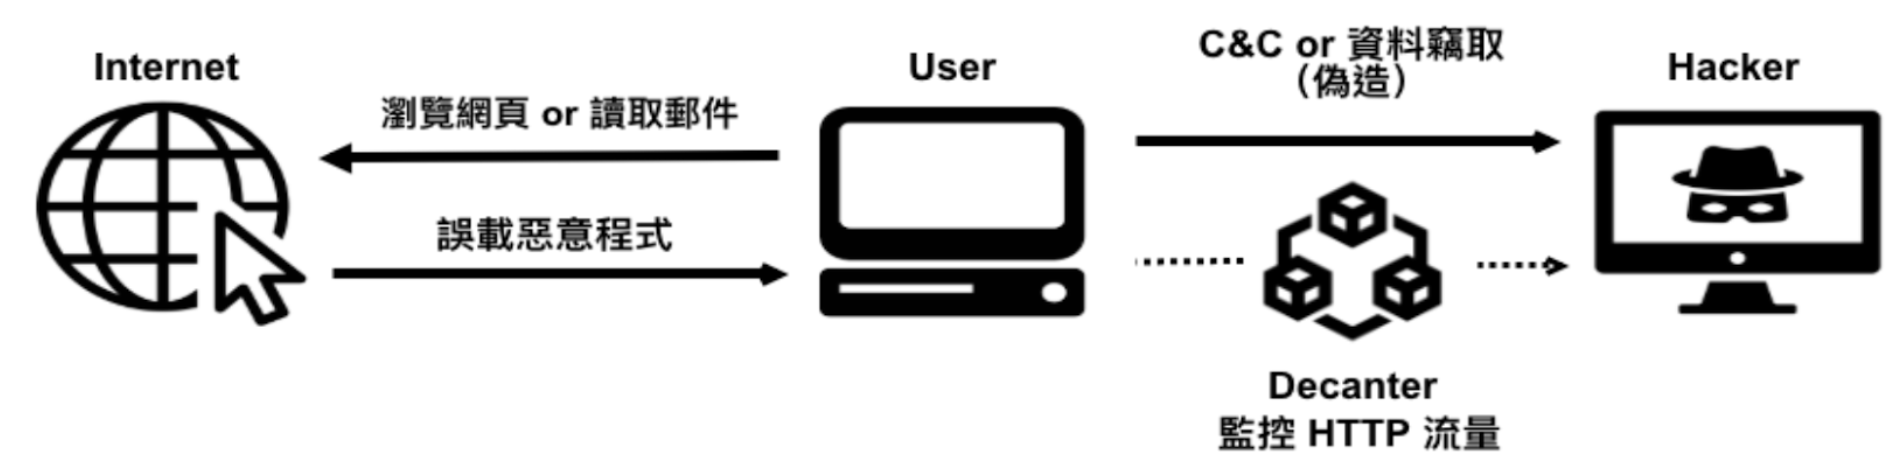
\includegraphics[width=250pt]{image/attack.png}
\caption{A process of attacking scenario}
\label{fig:attack}
\end{figure}


\begin{figure}[!tbp]
  \centering
  \subfloat[Normal Referrer Correlation Graph]{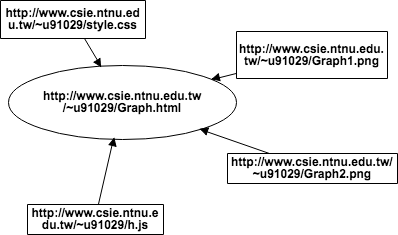
\includegraphics[width=0.25\textwidth]{image/normal.png}\label{fig:normal}}
  \hfill
  \subfloat[Malicious Referrer Correlation Graph]{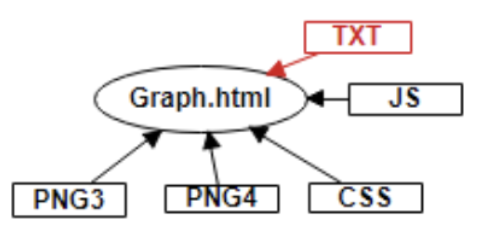
\includegraphics[width=0.25\textwidth]{image/malware.png}\label{fig:malware}}
  \caption{Difference between normal and malicious referrer correlation graph.}
\label{fig:length_count}
\end{figure}

Contributions of this work are briefly summarized as followings.

\begin{itemize}

\item {\bf Contribution 1}

Description here...

\item {\bf Contribution 2}

Description here...

\item {\bf Contribution 3}

Description here...

\end{itemize}